\documentclass[tikz,border=6pt]{standalone}
\usetikzlibrary{calc}
\begin{document}
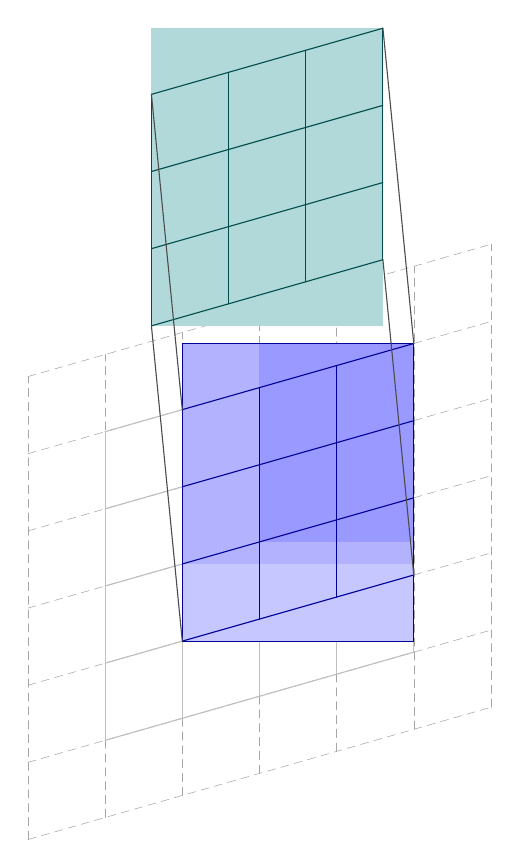
\begin{tikzpicture}[
  x={(0.98cm,0.28cm)},  % perspective basis (do not change independently)
  y={(0cm,0.98cm)},
  every path/.style={line cap=round, line join=round}
]

% ---------------- Bottom feature map ----------------
% Dashed context (same pitch as solid grid)
\foreach \i in {-1,...,5} {
  \draw[densely dashed, gray!70, very thin] (-1,\i) -- (5,\i);
  \draw[densely dashed, gray!70, very thin] (\i,-1) -- (\i,5);
}

% Solid 4x4 tile area
\foreach \i in {0,...,4} {
  \draw[gray!50] (0,\i) -- (4,\i);
  \draw[gray!50] (\i,0) -- (\i,4);
}

% Receptive field: 3x3 (upper-right of the 4x4)
\fill[blue!22] (1,1) rectangle (4,4);   % base fill
% (optional subtle shading similar to your image)
\fill[blue!30] (1,2) rectangle (4,4);
\fill[blue!40] (2,2) rectangle (4,4);
\draw[blue!60!black] (1,1) rectangle (4,4); % outline of the 3x3 RF
\foreach \i in {1,...,4} {
  \draw[blue!60!black] (1,\i) -- (4,\i);
  \draw[blue!60!black] (\i,1) -- (\i,4);
}

% ---------------- Top kernel plane ----------------
\coordinate (T) at (0.6,5.2); % vertical offset for the kernel plane

% 3x3 kernel (exactly aligned with RF corners)
\begin{scope}[shift={(T)}]
  \fill[teal!30] (0,0) rectangle (3,3);
  \foreach \i in {0,...,3} {
    \draw[teal!60!black] (0,\i) -- (3,\i);
    \draw[teal!60!black] (\i,0) -- (\i,3);
  }
\end{scope}

% ---------------- Corner-to-corner struts ----------------
\draw[black!70] (1,1) -- ($(T)+(0,0)$);
\draw[black!70] (4,1) -- ($(T)+(3,0)$);
\draw[black!70] (1,4) -- ($(T)+(0,3)$);
\draw[black!70] (4,4) -- ($(T)+(3,3)$);

\end{tikzpicture}
\end{document}
